% Created 2025-03-05 Wed 17:58
% Intended LaTeX compiler: pdflatex
\documentclass[11pt]{article}
\usepackage[utf8]{inputenc}
\usepackage[T1]{fontenc}
\usepackage{graphicx}
\usepackage{longtable}
\usepackage{wrapfig}
\usepackage{rotating}
\usepackage[normalem]{ulem}
\usepackage{amsmath}
\usepackage{amssymb}
\usepackage{capt-of}
\usepackage{hyperref}
\usepackage{minted}
\usepackage{siunitx}
\setlength{\parindent}{0em}
\newcommand{\sectionbreak}{\clearpage}
\newcommand{\subsectionbreak}{\clearpage}
\author{Nicholas Wee}
\date{\today}
\title{MA2071 E2.13 Report: Virtual Reality for Education}
\hypersetup{
 pdfauthor={Nicholas Wee},
 pdftitle={MA2071 E2.13 Report: Virtual Reality for Education},
 pdfkeywords={},
 pdfsubject={},
 pdfcreator={Emacs 30.1 (Org mode 9.7.11)}, 
 pdflang={English}}
\usepackage{calc}
\newlength{\cslhangindent}
\setlength{\cslhangindent}{1.5em}
\newlength{\csllabelsep}
\setlength{\csllabelsep}{0.6em}
\newlength{\csllabelwidth}
\setlength{\csllabelwidth}{0.45em * 4}
\newenvironment{cslbibliography}[2] % 1st arg. is hanging-indent, 2nd entry spacing.
 {% By default, paragraphs are not indented.
  \setlength{\parindent}{0pt}
  % Hanging indent is turned on when first argument is 1.
  \ifodd #1
  \let\oldpar\par
  \def\par{\hangindent=\cslhangindent\oldpar}
  \fi
  % Set entry spacing based on the second argument.
  \setlength{\parskip}{\parskip +  #2\baselineskip}
 }%
 {}
\newcommand{\cslblock}[1]{#1\hfill\break}
\newcommand{\cslleftmargin}[1]{\parbox[t]{\csllabelsep + \csllabelwidth}{#1}}
\newcommand{\cslrightinline}[1]
  {\parbox[t]{\linewidth - \csllabelsep - \csllabelwidth}{#1}\break}
\newcommand{\cslindent}[1]{\hspace{\cslhangindent}#1}
\newcommand{\cslbibitem}[2]
  {\leavevmode\vadjust pre{\hypertarget{citeproc_bib_item_#1}{}}#2}
\makeatletter
\newcommand{\cslcitation}[2]
 {\protect\hyper@linkstart{cite}{citeproc_bib_item_#1}#2\hyper@linkend}
\makeatother\begin{document}

\maketitle
\setcounter{tocdepth}{2}
\tableofcontents \clearpage\section{Abstract}
\label{sec:org2464ace}
The great pioneer of the modern concept of VR is Ivan Sutherland, who laid the foundational concept of what a VR device should look like. VR is used mainly as an entertainment and education tool, with it being very helpful in the visualisation of microscopic entities, such as cells and proteins, as well as complex mathematical concepts, such as the cross product of 3-dimensional vectors. It is also widely used for simulation training in preparation for a job, allowing users to make mistakes and fail safely in a virtual environment before needing to perform for real.
\section{Introduction}
\label{sec:org270a80f}
Before 1838, the panoramic paintings could be considered a primitive form of virtual reality, as it attempts to create the illusion of being somewhere where we are not \cslcitation{1}{[1]}.

\begin{figure}[htbp]
\centering
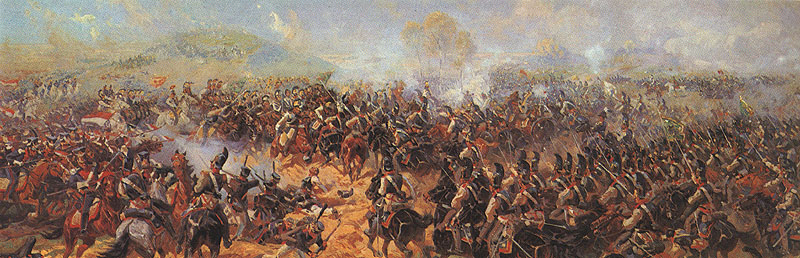
\includegraphics[width=.9\linewidth]{./images/battle-borodino.jpg}
\caption{The battle of borodino, 1812 \cslcitation{1}{[1]}.}
\end{figure}

 \newpage
\subsection{1838}
\label{sec:orge56830a}
In 1838, Charles Wheatstone, a professor of Experimental Philosophy at King's College created the stereoscope \cslcitation{2}{[2]}, which was a device that can be used to view 2-dimensional stereoscopic images, called stereograms, as 3-dimensional. This is done by enhancing the illusion of depth using stereopsis for 2-eyed vision \cslcitation{3}{[3]}.

\begin{figure}[htbp]
\centering
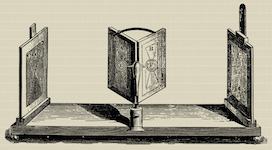
\includegraphics[height=12em]{./images/charles-wheatston-stereoscope.jpg}
\caption{The steoreoscope \cslcitation{1}{[1]}.}
\end{figure}
\subsection{1930s}
\label{sec:org6219c64}
Pygmalion's Spectacles, written by Stanley G. Weinbraum, was the first science fiction story to predict the existence of VR, by describing a pair of goggles that will allow the user to experience a virtual world through their senses \cslcitation{1}{[1]}.

\begin{figure}[htbp]
\centering
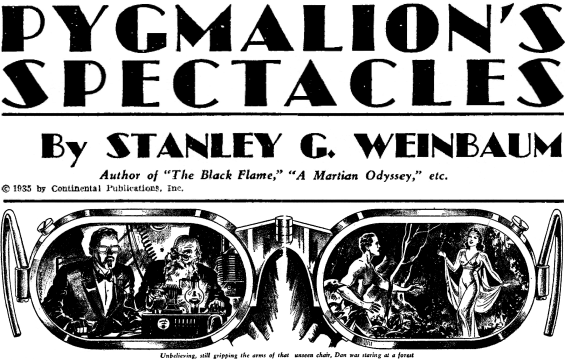
\includegraphics[height=12em]{./images/pygmallions-spectacles.png}
\caption{The cover of Pygmalion's Spectacles \cslcitation{1}{[1]}.}
\end{figure}
\subsection{1950s}
\label{sec:org868d230}
A cinematography called Morton Heilig created the Sensorama, which was created to stimulate all the senses. It came with smell generators, fans, a chair capable of vibration, stereo speakers, and of course, a stereographic 3D display. The device was created to fully immerse the viewer in the film \cslcitation{1}{[1]}.

\begin{figure}[htbp]
\centering
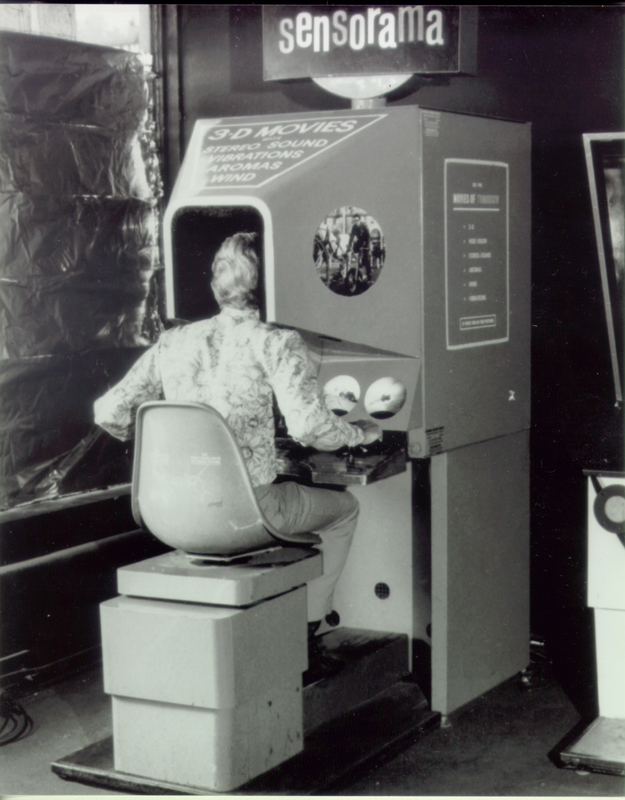
\includegraphics[height=14em]{./images/sensorama.jpg}
\caption{The Sensorama \cslcitation{4}{[4]}.}
\end{figure}
\subsection{1960}
\label{sec:org96e950c}
Morton Heilig creates the first VR head-mounted display, called the Telesphere Mask. The headset provided stereoscopic 3D and wide vision with stereo sound \cslcitation{1}{[1]}.

\begin{figure}[htbp]
\centering
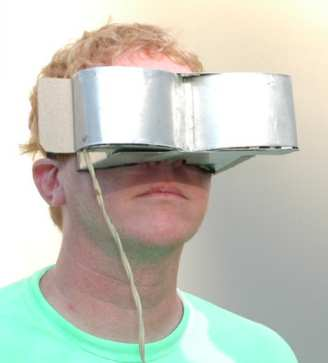
\includegraphics[height=13em]{./images/telesphere-mask.jpg}
\caption{The Telesphere Mask \cslcitation{4}{[4]}.}
\end{figure}
\subsection{1961}
\label{sec:orgb4d1b3e}
Comeau and Bryan developed the first motion tracking head-mounted display, called the Headsight. It featured binocular video screens and a magnetic motion tracking system which is linked to a closed circuit camera. The device was developed for military applications, particularly to immersively view dangerous situations \cslcitation{1}{[1]}.
\subsection{1965}
\label{sec:orgb6ac90c}
Ivan Sutherland describes the "Ultimate Display" concept, which could simulate reality to the point where it is impossible to tell the difference from actual reality. The "Ultimate Display" should include a realistic virtual world viewed through a head-mounted display that can be interacted with the user's senses, and provides sonic and tactile feedback. It should also include hardware to continuously generate and respond to the user's action in real time \cslcitation{1}{[1]}.

 \newpage
\subsection{1968}
\label{sec:orgd79e52c}
Ivan Sutherland creates the Sword of Damocles, which is the first head-mounted display that is connected to a computer instead of a camera, unlike the Headsight. However, the contraception was extremely bulky and heavy, and hence had to be hung from the ceiling since it would be too heavy for anyone to comfortably wear. The user also needed to be strapped in to the device to provide support for the heavy mechanism \cslcitation{1}{[1]}.

\begin{figure}[htbp]
\centering
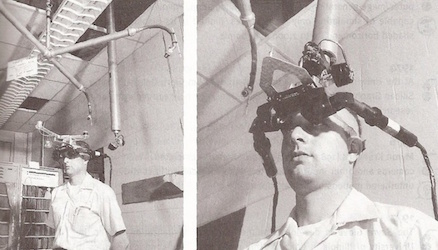
\includegraphics[width=.9\linewidth]{./images/ivan-sword-of-damocles.jpg}
\caption{The Sword of Damocles in action \cslcitation{1}{[1]}.}
\end{figure}
\subsection{1969}
\label{sec:orgfc16078}
Myron Kruegere, a virtual reality computer artist, creates "Artificial Reality", which is a series of computer-generated environments that respond to the user's input \cslcitation{1}{[1]}.
\subsection{1975}
\label{sec:org673e2a9}
Myron Kruegere creates the VIDEOPLACE system, which is widely regarded as the first interactive AR system. It uses a mix of cameras, light projection, computer-generation and screens to measure user's position. It is considered an AR system as it projects to a screen rather than having the user wear a head-mounted display \cslcitation{1}{[1]}.
\subsection{1977}
\label{sec:orgce03e4b}
MIT creates the Aspen Movie Map, which allowed users to explore Aspen, Colorado in a virtual tour. Videos were filmed from a moving car to create the illusion of walking through the city \cslcitation{1}{[1]}, \cslcitation{5}{[5]}.

\begin{figure}[htbp]
\centering
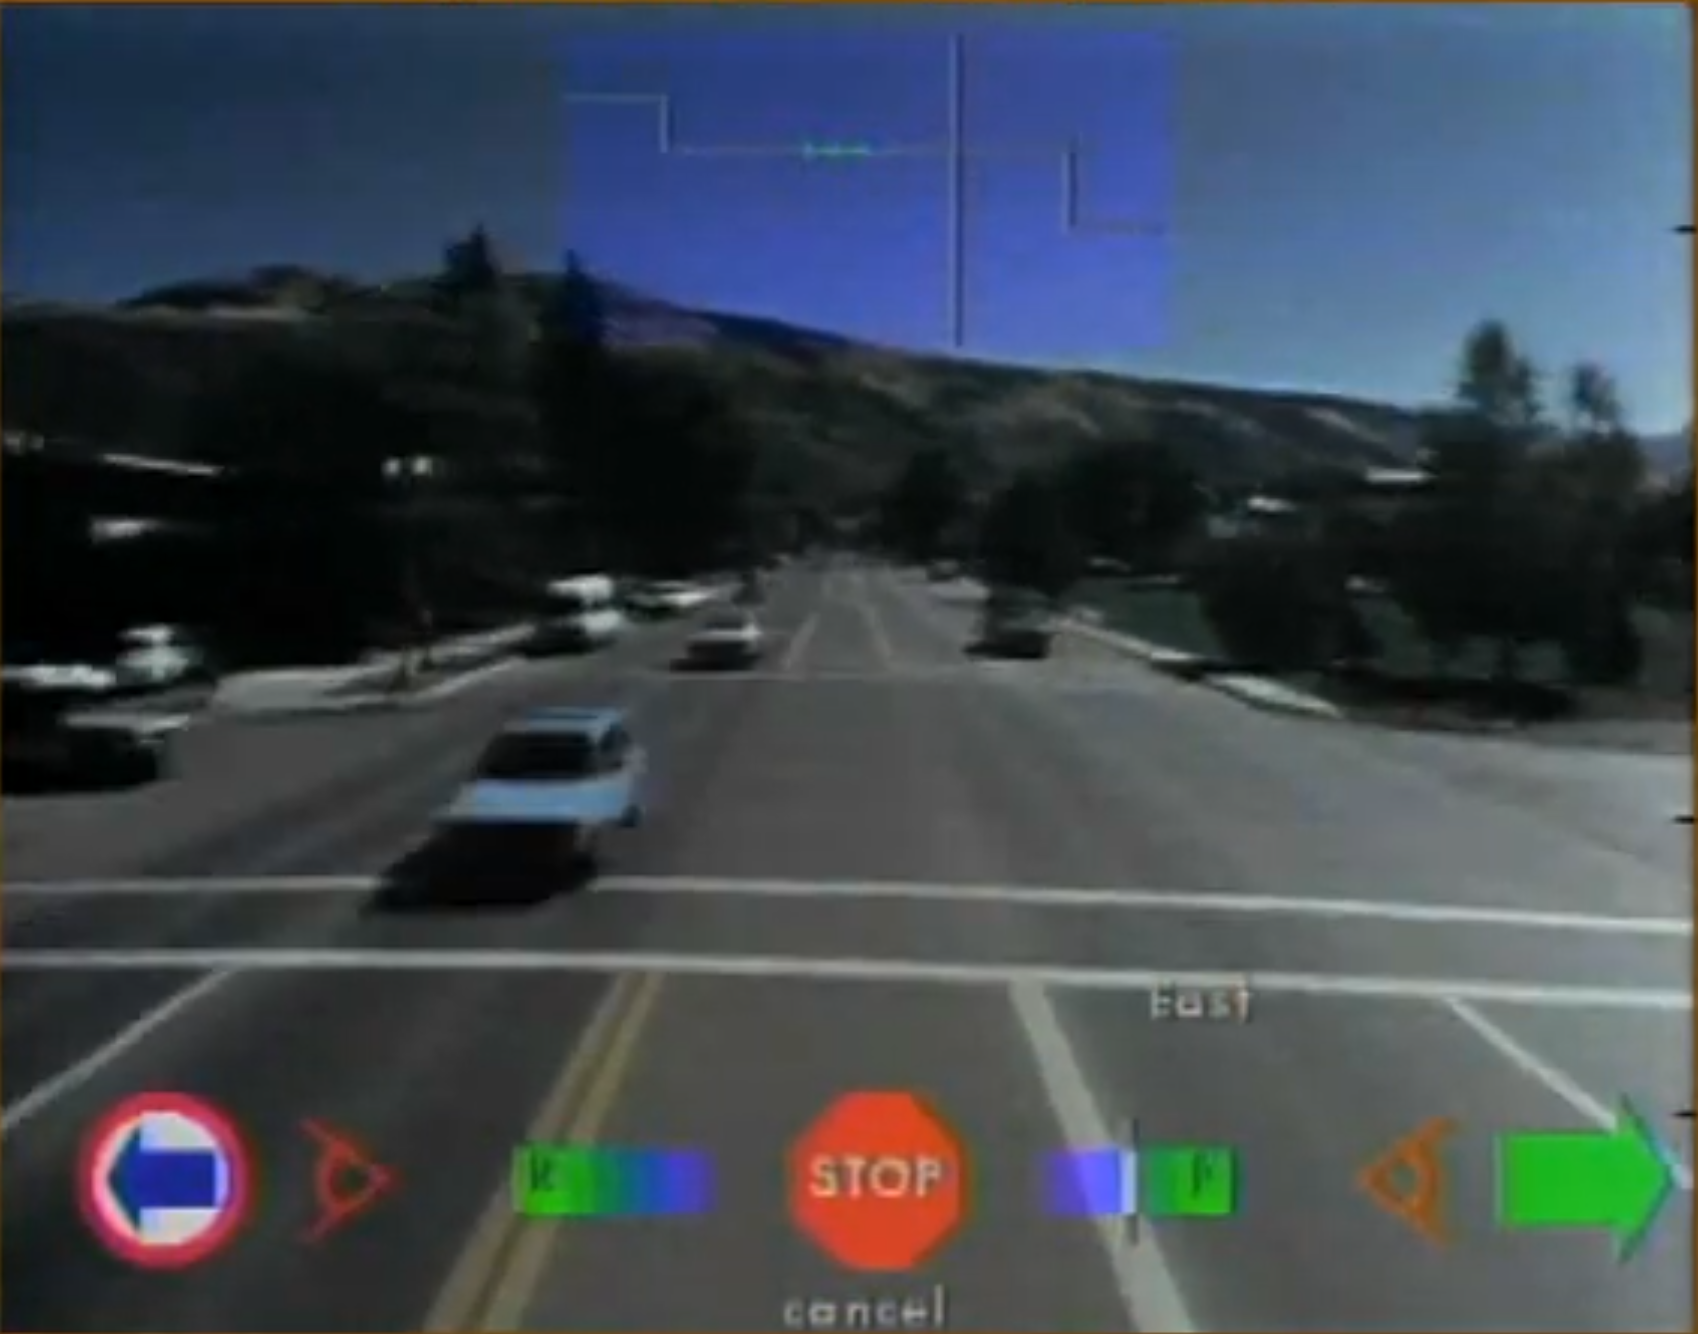
\includegraphics[height=18em]{./images/aspen-movie-map.png}
\caption{The Aspen Movie Map \cslcitation{6}{[6]}}
\end{figure}
\subsection{1982}
\label{sec:org625267c}
Daniel Sandlin and Thomas DeFanti create finger-tracking gloves called "Sayre" gloves, which used optical sensors to detect finger movement \cslcitation{1}{[1]}.
\subsection{1985}
\label{sec:orge01c7ac}
Jaron Lanier and Thomas Zimmerman found Visual Programming Lab Research, which is the first ever company to sell head-mounted displays and gloves. The "data glove" name comes from their product, the DataGlove \cslcitation{1}{[1]}.
\subsection{1987}
\label{sec:org741580d}
Virtual reality, or VR, is coined as a term by Jaron Lanier. His company, Visual Programming Lab Research, created a great many devices for the purpose of virtual reality, such as the DataGlove and the EyePhone head-mounted display \cslcitation{1}{[1]}.
\section{Literature review}
\label{sec:orgc47e08b}
As VR technology becomes more powerful and more affordable, the VR is increasingly being applied in education as a teaching aid to help students in understanding difficult concepts better. It is also used to put students in exceptional circumstances to teach them how to react or behave in those circumstances, without actually being in those circumstances.
\subsection{Purpose of VR in education}
\label{sec:orgd399478}
Currently, VR is being applied in education for 4 different purposes. They are simulation, training, access of limited resources, and facilitating distance learning \cslcitation{7}{[7]}.
\subsubsection{Simulation}
\label{sec:orgf5760de}
One of the biggest uses of VR for education is due to its ability to simulate life-like situations and scenarios that would otherwise be dangerous or impractical \cslcitation{8}{[8]}, \cslcitation{9}{[9]}, \cslcitation{10}{[10]}. For example, Sun's paper \cslcitation{8}{[8]} creates a 3D virtual reality model of the sun and the moon for e-learning at elementary schools, which would be infeasible in reality. VR is usually also much cheaper than bringing such experiences in reality, as it would usually entail expensive overseas trips that schools will not have the budget for \cslcitation{7}{[7]}.

Boyles found that AR is used widely in electrical engineering, with applications such as ElectARManual, ELECT3D and ElectAR notes. He also found virtual and augmented reality to be used widely in various scientific fields, such as visualisation of chemical reactions in chemistry, visualising respiration and meiosis in biology, and to explore the solar system in astronomy \cslcitation{11}{[11]}.

 \newpage
\subsubsection{Training}
\label{sec:org8173f60}
Kavanagh found that 58\% of simulations found in his review were used for training purposes \cslcitation{7}{[7]}, and included various applications such as flight simulators \cslcitation{9}{[9]}, chemical engineering \cslcitation{10}{[10]} and construction \cslcitation{12}{[12]}.

He also found that VR is very commonly used to simulate medical activities for training purposes, especially surgery, but it can also be used to simulate other medical activities such as rehabilitation \cslcitation{7}{[7]}. For example, Nolin used a virtual classroom to assess children with attention deficit disorders \cslcitation{13}{[13]}.

Another common use case of VR is for pilot training, as virtual flights can be carried out similarly to actual piloting, since piloting is highly computerised in the modern age \cslcitation{7}{[7]}. This use of VR allows the pilot to train as much as they want, and make as many mistakes as they want, as such simulations do not pose any danger to the pilots \cslcitation{9}{[9]}, \cslcitation{14}{[14]}. Similarly for the medical field, there are no patients that suffer from a virtual surgery.
\subsubsection{Access limited resources}
\label{sec:orgcbce944}
In virtual reality, resources are theoretically infinite, and hence, it can be used to simulate the access of limited resources. For example, Rahim simulated a commercial milk powder processing plant for students of chemical and process engineering, as visiting such plants was difficult due to availability and safety regulations \cslcitation{10}{[10]}. Another example would be to have art or archaeological pieces which are geographically separated be brought together into the virtual world where the user can experience it in one place \cslcitation{15}{[15]}.
\subsubsection{Distance learning}
\label{sec:orga21b660}
Distance learning refers to experiential learning from a distance, without the need to be in a particular location, which is made possible through virtual reality. For example, Chang created a system to teach users with cerebral palsy how to independently perform rehabilitation exercises. This was much better than video tutorials as the Kinect motion-sensing devices could provide real-time feedback regarding the validity of their form based off of their joint angles \cslcitation{16}{[16]}.

 \newpage
\section{Fundamentals of VR}
\label{sec:org9c82a15}
In VR and AR, there are 4 characteristics which are important to have an immersive experience, namely:
\begin{itemize}
\item Fidelity modelling and simulation
\item Realistic and immersive visualisation
\item Real-time interaction
\item Natural user interface
\end{itemize}

The experience in VR and AR needs to be as close to the actual physical world as possible, so models and simulations inside the virtual world should behave similarly to that of the physical world. Interactions in the virtual world have to be real-time, and interfaces to the virtual world should be similar to how a person interacts with the physical world, making use of their senses.
\subsection{Fidelity modelling and simulation}
\label{sec:org02a33f9}
Virtual worlds should ideally be as close to the physical world as possible, to make sure the player feels immersed in the virtual world. The ideal would be to have a world where the virtual world and the real world are indistinguishable, like in the movie called "The Matrix". As such, 3D models and physics simulations in the virtual world need to be high fidelity to create the illusion of reality for the player and have them be engrossed and fully immersed in the experience. Simulated smell and taste would be ideal too, but currently, those aren't the focus at the moment for consumer VR headsets.
\subsection{Realistic and immersive visualisation}
\label{sec:org390d1dc}
This is quite similar to the point above about modelling and simulation, but it refers more specifically to visualisations rather than the modelling of objects and the simulation of physics in the virtual world. Similar to modelling and simulation, visualisations in a virtual world should look realistic to keep the user engrossed in the world and to not break their immersion. Visuals in the virtual world should follow the design and visuals of real world objects, so that the transition between the real world into the virtual world is as smooth as possible, and ideally the user should not notice a difference if the visualisations are realistic enough.
\subsection{Real-time interaction}
\label{sec:orgaab2bc2}
Once again, because virtual worlds should behave like the real physical world, all interactions in the visual world should be near instant and have immediate feedback, as that is how the real world works. Real-time interactions keep the user immersed in the virtual world. Ideally the user would also get tactile feedback and sonic feedback from the items they interact with, just like in the real world, but it is also not a focus at the moment for consumer VR headsets.
\subsection{Natural user interface}
\label{sec:orgba47636}
A natural user interface means that the user should interact with the world using his senses instead of relying on a controller to control their movements in the virtual world. Ideally, the user would interact with all objects in the virtual world just like he would in the real world. Hence, interactions in the virtual world will need to be designed around the user using his sight, his touch and even his voice or the sounds he makes to interact with objects in the virtual world. Currently, most VR headsets rely on motion and gesture tracking to figure out the action the user is taking and response to it. However, this way of emulating touch interaction has a lot of issues current, mainly with the camera location and the hand obscuring fingers which makes the controls go haywire, which is not idea for an intuitive and natural user interface that doesn't need to be learnt.
\section{Experiment}
\label{sec:org2412c4f}
Overall, I found the experiments to be quite interesting, and learnt that different VR games will implement different control schemes, some better than others. The current technology for a natural control scheme isn't currently ideal, as a lot of my classmates found it difficult to figure out the controls in VR as they don't really work all that well and have trouble in tracking the motion of the hand. When the back of the hand obscures the fingers, the motion tracking goes haywire and things don't work well, and it happens very often. A controller might be still be a more intuitive control interface compared to using motion tracking with a camera for now.

 \newpage
\subsection{Virtual cells}
\label{sec:org9ed8021}
This experiment was about seeing cell parts, such as the mitochondria, Golgi body and the endoplasmic reticulum. It was quite fun to use my hands to manipulate the cells, but I was somewhat disappointed that the simulations were not more detailed.

\begin{figure}[htbp]
\centering
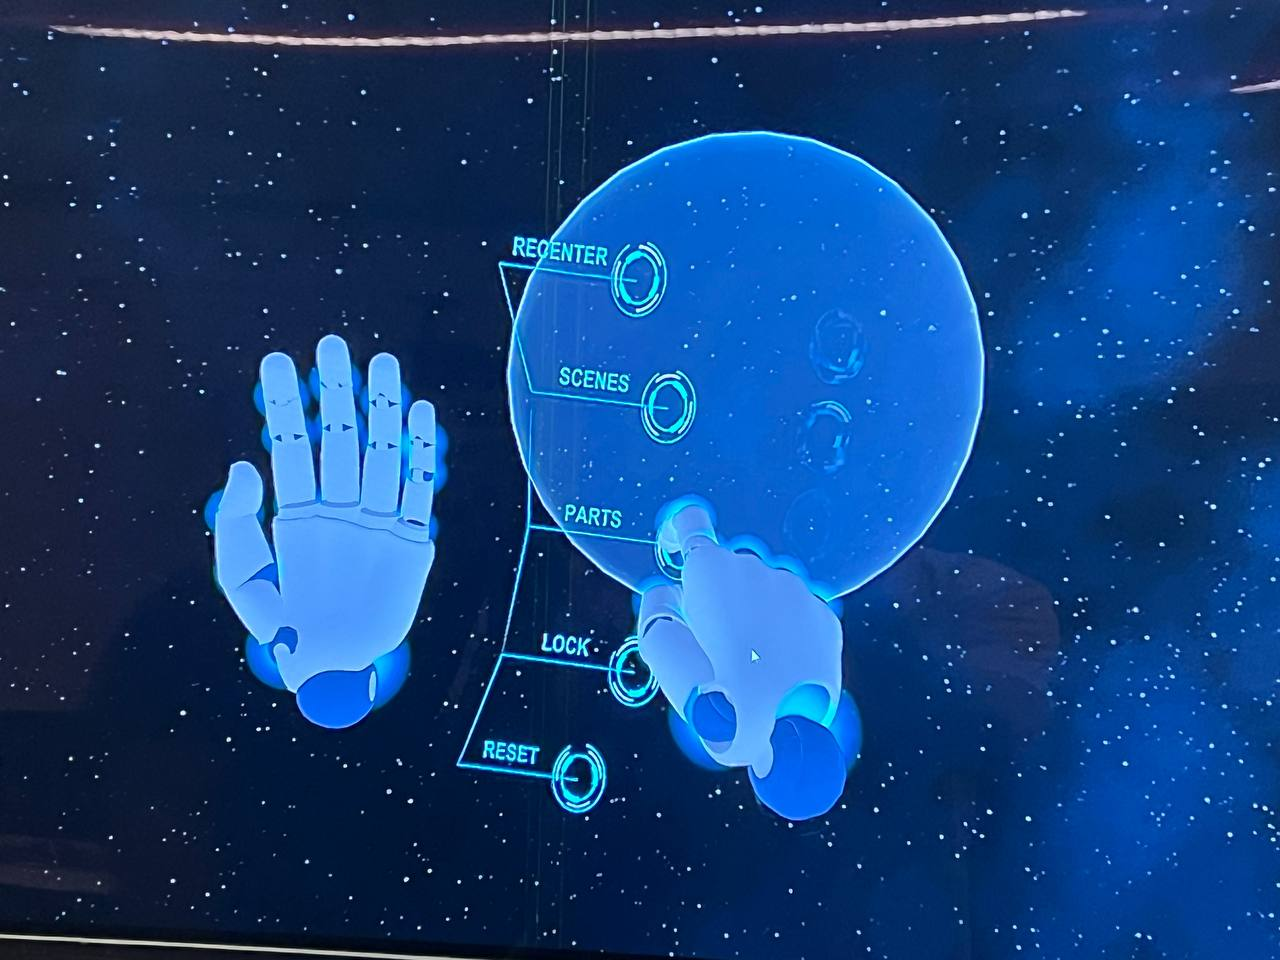
\includegraphics[height=15em]{./images/virtual-cell-game-menu.jpg}
\caption{The menu.}
\end{figure}

\begin{figure}[htbp]
\centering
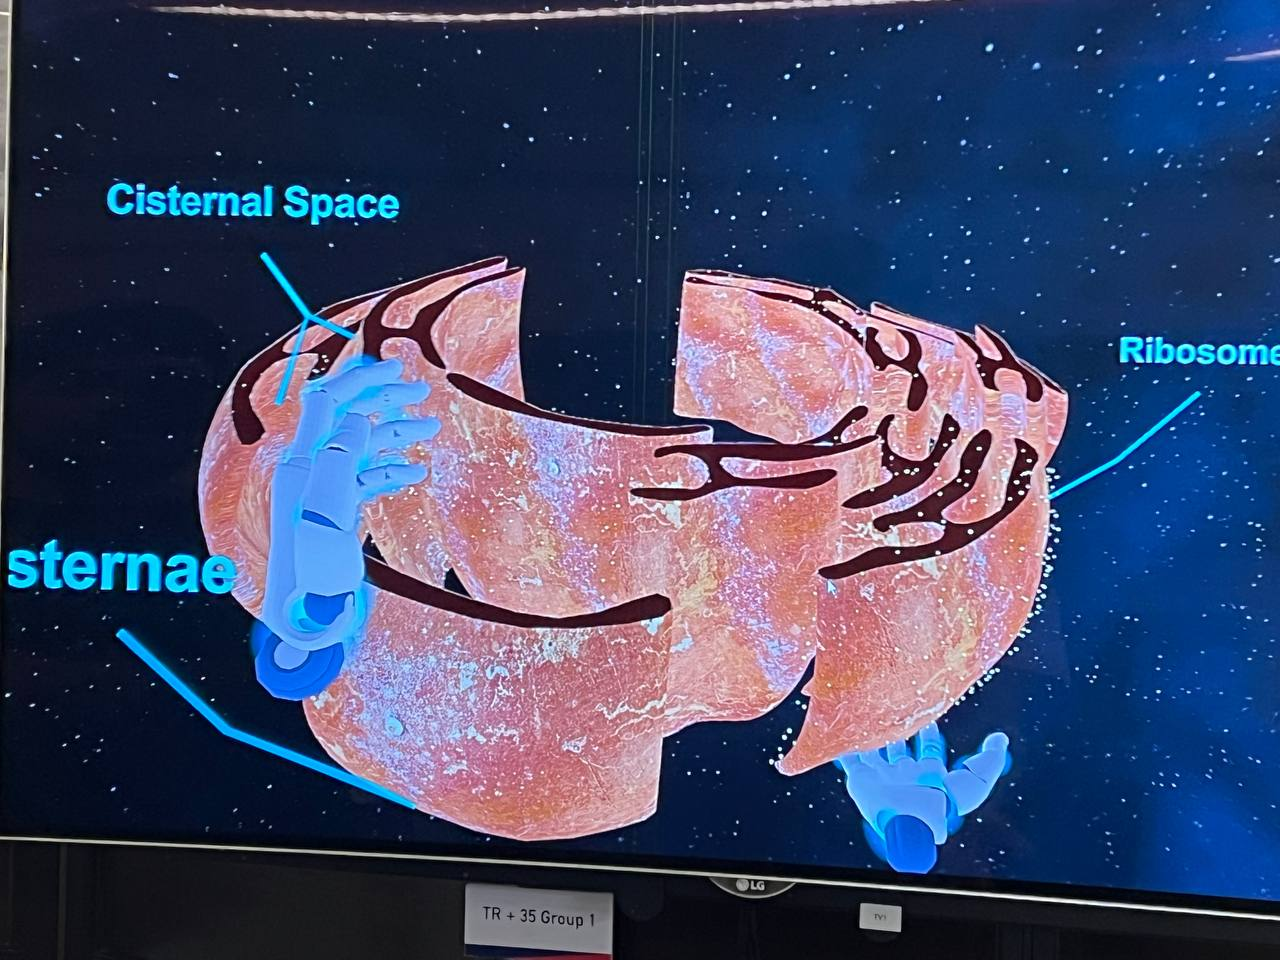
\includegraphics[height=15em]{./images/endoplasmic-reticulum.jpg}
\caption{The VR simulation of an endoplasmic reticulum.}
\end{figure}

\begin{figure}[htbp]
\centering
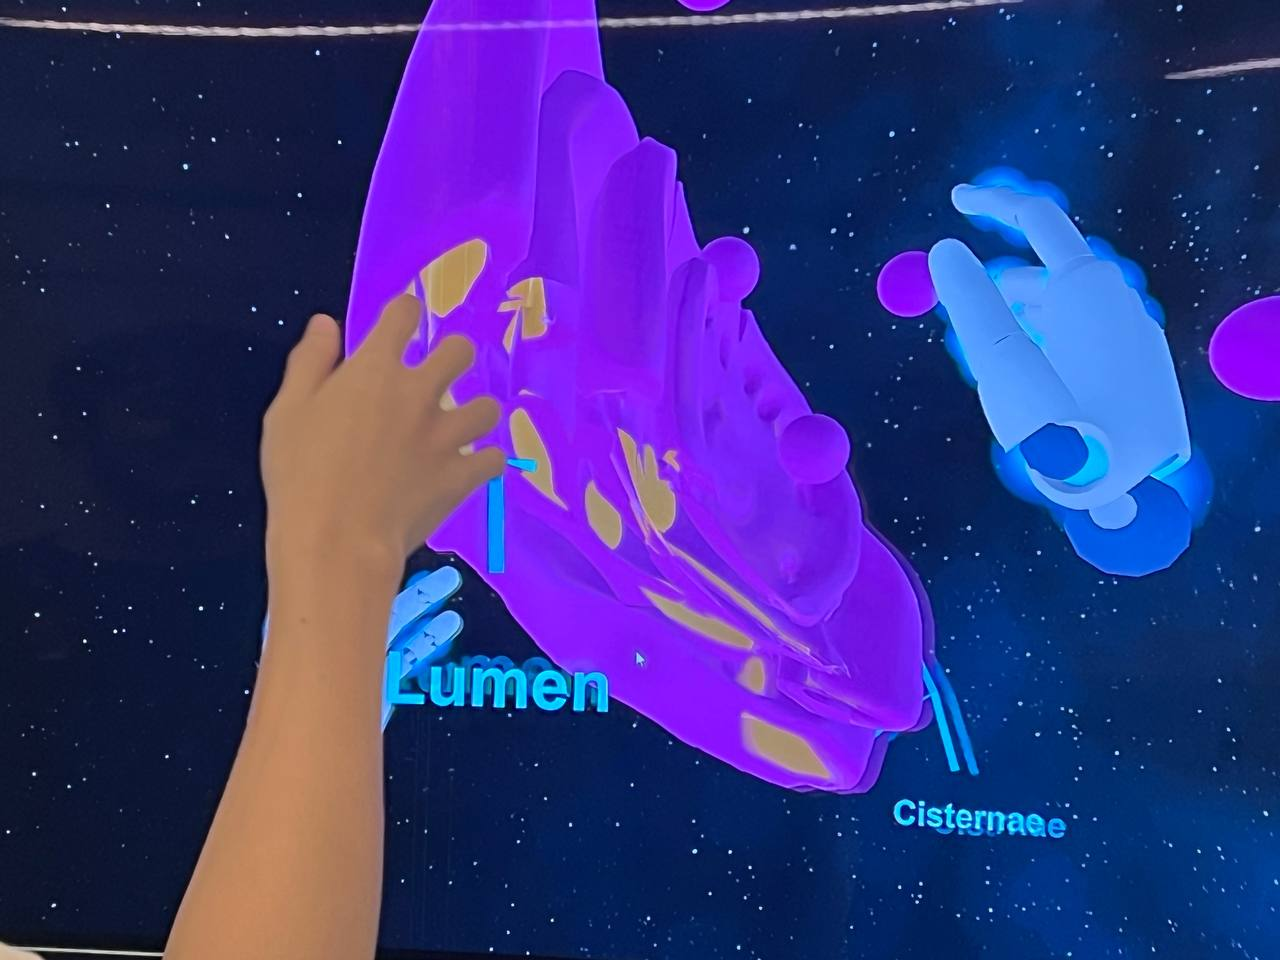
\includegraphics[height=15em]{./images/golgi-body.jpg}
\caption{The VR simulation of a Golgi body.}
\end{figure}
\subsection{Virtual F1}
\label{sec:org59769a3}
This experiment was about putting together an F1 car and seeing it drive through an obstacle course. The controls in this one weren't as polished as the virtual cell game, and the pinching gesture didn't work half the time due to the fingers being obscured by the back of the hand. It was quite interesting to see how an F1 car looks on the inside though.

\begin{figure}[htbp]
\centering
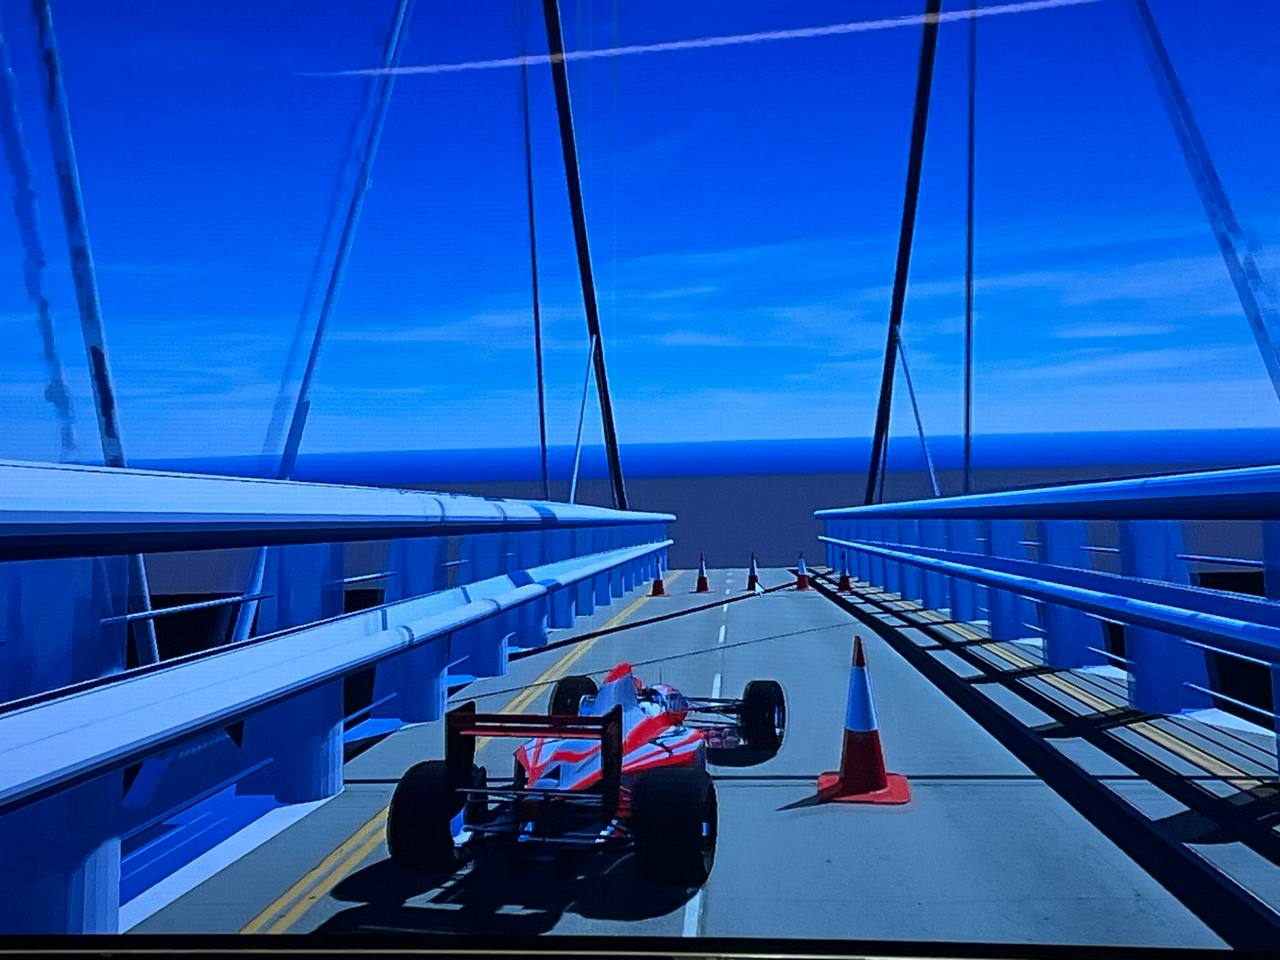
\includegraphics[height=15em]{./images/f1-car-driving-through-obstacles.jpg}
\caption{The F1 car driving through obstacles after being assembled.}
\end{figure}
\subsection{Virtual vectors}
\label{sec:org20653eb}
This experiment was about visualising the result of a cross product of two vectors. This experiment also included a new kind of control scheme, which is eye tracking and focus, but I didn't find it to work well compared to hand gestures. It wasn't obvious that you had to focus on a spot to have something happen, and it is also a bit difficult to keep your body and eyes still to have the action registered. However, the use of VR seems quite useful in the teaching of vectors, as it makes it much easier to visualise and gain an intuitive understanding of how the cross product work. I wonder if it would be possible to use VR to visualise quaternions, as quaternions are far more difficult to visualise and imagine, since we are only capable of perceiving 3 dimensions, while quaternions are 4-dimensional objects. Perhaps a 3-dimensional stereographic projection of quaternions may be possible in VR.

\begin{figure}[htbp]
\centering
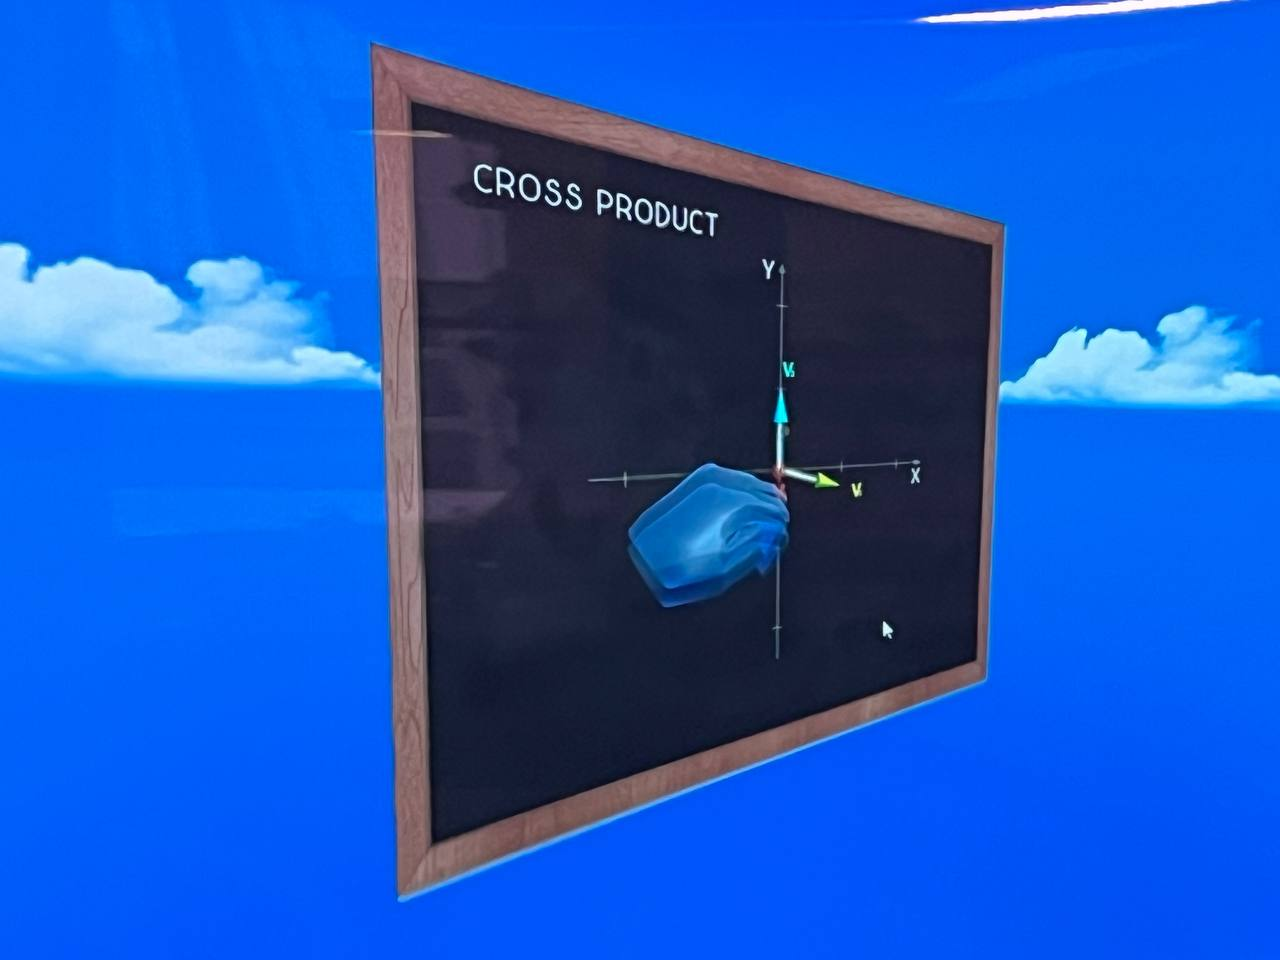
\includegraphics[height=20em]{./images/dragging-the-vectors.jpg}
\caption{Dragging the vectors around to change the cross product vector.}
\end{figure}

\begin{figure}[htbp]
\centering
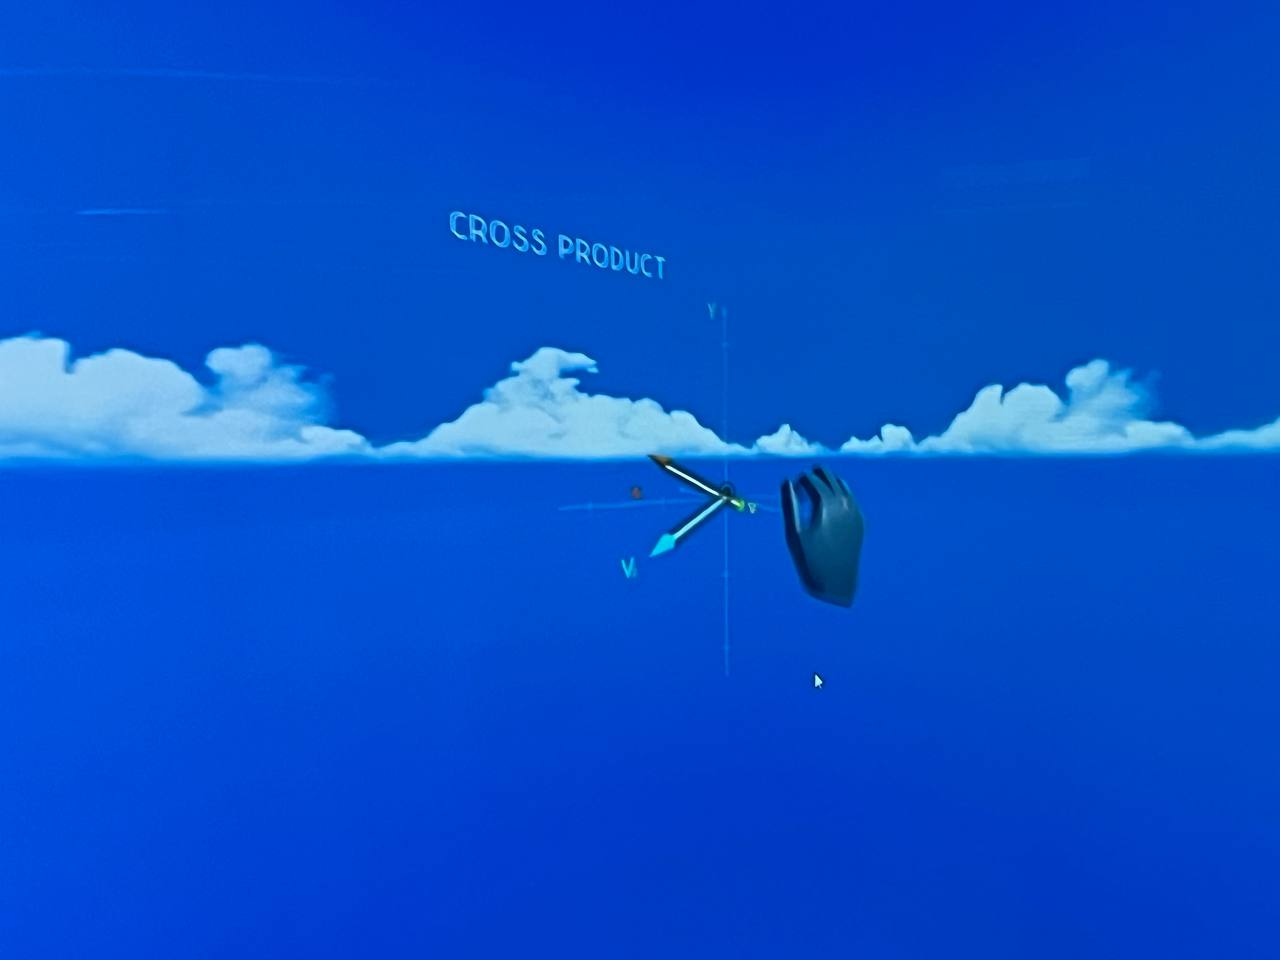
\includegraphics[height=20em]{./images/dragging-the-vectors-no-blackboard.jpg}
\caption{Manipulating the vectors with the blackboard removed.}
\end{figure}

\begin{figure}[htbp]
\centering
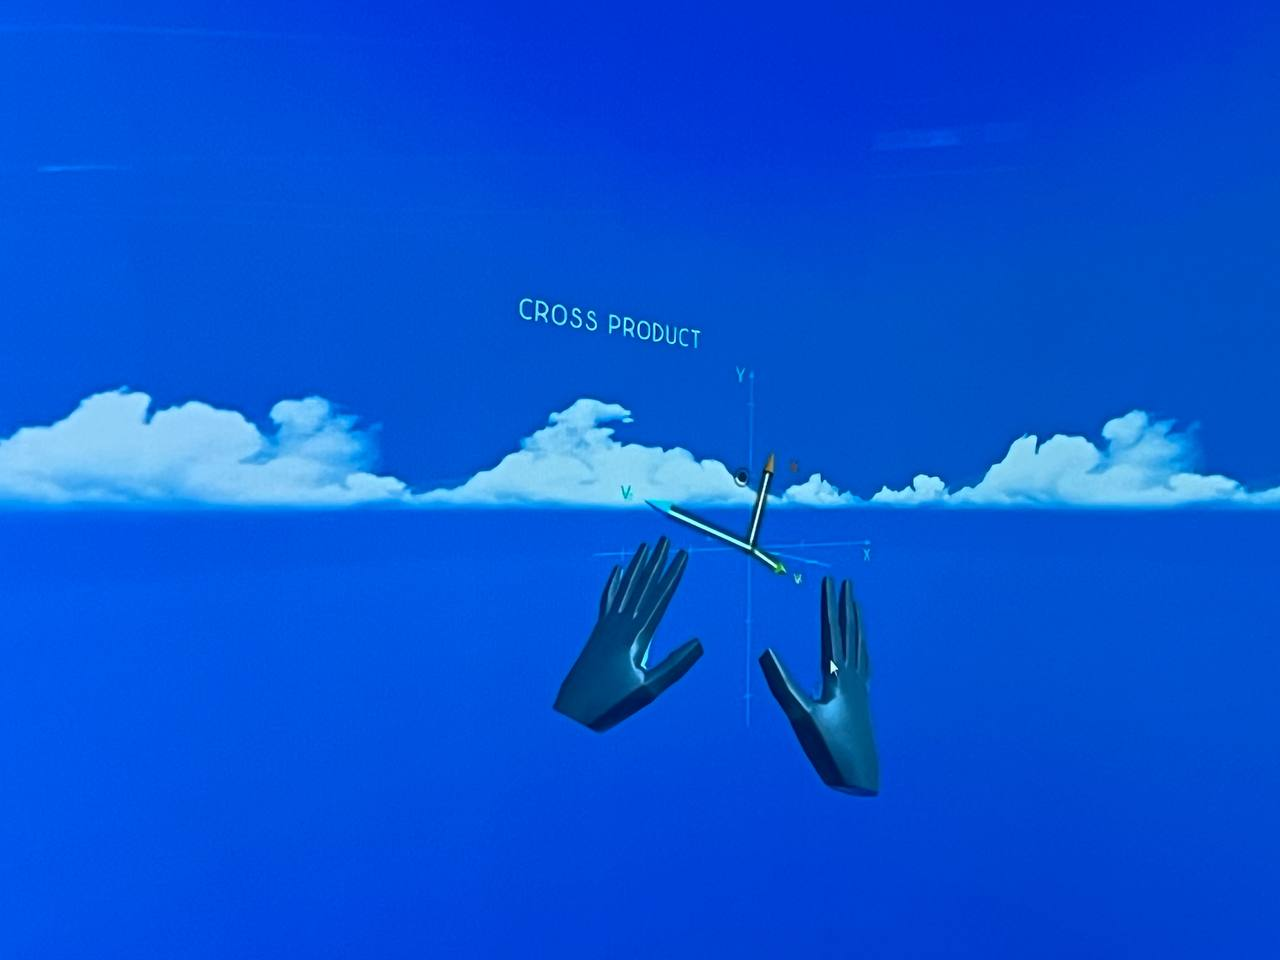
\includegraphics[height=20em]{./images/cross-product-vectors.jpg}
\caption{The cross product vectors.}
\end{figure}

 \newpage
\section{Discussion and conclusion}
\label{sec:orgbc87c15}
As discussed in the literature review above, virtual and augmented reality has been used in many applications for education. With VR technology becoming cheaper and more widespread, it is likely that educators and schools alike will increase adoption of this technology to provide higher quality education at lower cost, such as experiential learning through virtual worlds and the ability to visit places that are difficult or even impossible to reach in reality.
\subsection{Pros}
\label{sec:org2ba7036}

\subsubsection{Personalised learning}
\label{sec:orgdb3cf20}
The main benefit of VR is that learning can be easily personalised to the students, as it is easy to let the student have a large amount of control over the virtual world and let them explore and learn at their own pace. Virtual reality also allows students to repeat lessons as many times as they want to improve their understanding, without affecting their classmates \cslcitation{7}{[7]}.
\subsubsection{Deeper learning}
\label{sec:org1ef489c}
In VR, students are able to learn via doing, instead of just memorising for tests. The ability to visualise complex and abstract concepts in virtual reality can also help students understand the concepts being taught at a deeper level. VR is also better for learn practical skills, such as doing surgery in medical fields, or doing handyman work for engineering, as students will actually perform the task and get feedback similar to that of performing the task in the real world, which would better understanding and improve muscle memory \cslcitation{7}{[7]}.

 \newpage
\subsection{Cons}
\label{sec:org23503d1}

\subsubsection{Cost}
\label{sec:orgaf02245}
Virtual reality experiences are not cheap to build, as it takes a lot of time and effort to create a custom, tuned experience for a specific domain. 3D modelling and programming a game in 3D are difficult tasks that take a lot of time to complete, and also require quite a lot of domain knowledge to ensure that the simulation is sufficiently realistic and mimics real world situations. Moreover, from my experience with the experiments, the natural user interfaces employed by VR don't seem to have built-in abstractions, such as standard API calls for developers to use, which means each developer has to roll their own implementation of these natural user interfaces, which makes for an inconsistent experience throughout different VR experiences and games.
\subsubsection{Insufficient realism}
\label{sec:org1cd5c5e}
Current virtual reality technology is still not at the point where it can perfectly simulate everything in the real world, so there are breaks in immersion due to poorly implemented user interfaces. One example would be the issue of the hand covering the fingers, causing the motion tracking camera that tracks hand and finger motion to go haywire when it cannot see the fingers. Such breaks in immersion can detract from the learning experience, as it distracts students from the actual game or experience. Insufficient realism in simulating real world experiences could result in the learnings being of limited value when applied to the real world. It could also result in bad situations in the real world if the simulation turns out to be incorrect, and has ingrained responses in users that are inappropriate or even dangerous to perform in the real world.

 \newpage
\section{References}
\label{sec:org4f4d2e3}
\begin{cslbibliography}{0}{0}
\cslbibitem{1}{\cslleftmargin{[1]}\cslrightinline{V. Society, “History of virtual reality,” Jan. 2020. Available: \url{https://www.vrs.org.uk/virtual-reality/history.html}}}

\cslbibitem{2}{\cslleftmargin{[2]}\cslrightinline{K. College, “Charles wheatstone: The father of 3d and virtual reality technology,” Oct. 2016. Available: \url{https://www.kcl.ac.uk/charles-wheatstone-the-father-of-3d-and-virtual-reality-technology-2}}}

\cslbibitem{3}{\cslleftmargin{[3]}\cslrightinline{R. Lazarus, “3D vision is more important than you think,” Jul. 2021. Available: \url{https://www.optometrists.org/vision-therapy/vision-therapy-for-lazy-eye/7-signs-your-child-might-have-a-lazy-eye/stereopsis-more-than-3d-vision/}}}

\cslbibitem{4}{\cslleftmargin{[4]}\cslrightinline{H. Foundation, “Usc hmh foundation moving image archive ’ morton heilig : Inventor vr,” Jan. 2023. Available: \url{https://hmharchive.com/morton-heilig-inventor-vr/}}}

\cslbibitem{5}{\cslleftmargin{[5]}\cslrightinline{Wikipedia, “Aspen movie map,” Jul. 2024, \textit{Wikimedia Foundation}. Available: \url{https://en.wikipedia.org/wiki/Aspen_Movie_Map}}}

\cslbibitem{6}{\cslleftmargin{[6]}\cslrightinline{M. Naimark, “Aspen interactive movie map,” Feb. 2016, \textit{YouTube}. Available: \url{https://www.youtube.com/watch?v=2Ytd12d6qNw}}}

\cslbibitem{7}{\cslleftmargin{[7]}\cslrightinline{S. Kavanagh, A. Luxton-Reilly, B. Wuensche, and B. Plimmer, “A systematic review of virtual reality in education,” \textit{Themes in science and technology education}, vol. 10, no. 2, pp. 85–119, 2017.}}

\cslbibitem{8}{\cslleftmargin{[8]}\cslrightinline{K.-T. Sun, C.-L. Lin, and S.-M. Wang, “A 3-d virtual reality model of the sun and the moon for e-learning at elementary schools,” \textit{International journal of science and mathematics education}, vol. 8, pp. 689–710, 2010.}}

\cslbibitem{9}{\cslleftmargin{[9]}\cslrightinline{W. Wei, L. Dongsheng, and L. Chun, “Fixed-wing aircraft interactive flight simulation and training system based on xna,” in \textit{2013 International conference on virtual reality and visualization}, IEEE, 2013, pp. 191–198.}}

\cslbibitem{10}{\cslleftmargin{[10]}\cslrightinline{E. Abdul Rahim \textit{et al.}, “A desktop virtual reality application for chemical and process engineering education,” in \textit{Proceedings of the 24th australian computer-human interaction conference}, 2012, pp. 1–8.}}

\cslbibitem{11}{\cslleftmargin{[11]}\cslrightinline{B. Boyles, “Virtual reality and augmented reality in education,” \textit{Center for teaching excellence, united states military academy, west point, ny}, vol. 67, 2017.}}

\cslbibitem{12}{\cslleftmargin{[12]}\cslrightinline{A. Z. Sampaio and L. Viana, “Virtual reality used as a learning technology: Visual simulation of the construction of a bridge deck,” in \textit{2013 8Th iberian conference on information systems and technologies (cisti)}, IEEE, 2013, pp. 1–5.}}

\cslbibitem{13}{\cslleftmargin{[13]}\cslrightinline{P. Nolin \textit{et al.}, “Clinicavr: Classroom-cpt: A virtual reality tool for assessing attention and inhibition in children and adolescents,” \textit{Computers in human behavior}, vol. 59, pp. 327–333, 2016.}}

\cslbibitem{14}{\cslleftmargin{[14]}\cslrightinline{R. L. Page, “Brief history of flight simulation,” \textit{Simtect 2000 proceedings}, pp. 11–17, 2000.}}

\cslbibitem{15}{\cslleftmargin{[15]}\cslrightinline{I. Angeloni, F. Bisio, A. De Gloria, D. Mori, C. Capurro, and L. Magnani, “A virtual museum for flemish artworks. a digital reconstruction of genoese collections,” in \textit{2012 18Th international conference on virtual systems and multimedia}, IEEE, 2012, pp. 607–610.}}

\cslbibitem{16}{\cslleftmargin{[16]}\cslrightinline{Y.-J. Chang, C.-C. Wang, Y.-S. Luo, and Y.-C. Tsai, “Kinect-based rehabilitation for young adults with cerebral palsy participating in physical education programs in special education school settings,” in \textit{Edmedia+ innovate learning}, Association for the Advancement of Computing in Education (AACE), 2014, pp. 792–795.}}

\end{cslbibliography}
\end{document}
